\subsection{信号的数学基础}

\subsubsection{欧拉(Euler)公式}

\begin{definition}[实值信号与复值信号]
    如果信号的取值是实数,则称为\bd{实值信号},简称\bd{实信号}。
    如果信号的取值是复数,则称为\bd{复值信号},简称\bd{复信号}。
\end{definition}

\begin{theorem}[欧拉公式]
    对于任意的 $\theta \in \set{R}$,都有以下的恒等式成立:
    \begin{align*}
        \mathe^{\mathi \theta} = \cos \theta + \mathi \sin\theta.
    \end{align*}

    特别地,当 $\theta = \pi$ 时,有 $\mathe^{\mathi\pi} + 1 = 0$。
\end{theorem}

\begin{proof}
    (欧拉公式的泰勒级数法证明) 分别将 $\mathe^x, \sin x, \cos x$ 进行泰勒(Taylor)展开,得:
    \begin{align*}
        \mathe^x &= \sum_{k = 0}^{+\infty}\frac{x^k}{k!}, \\
        \sin x   &= \sum_{k = 0}^{+\infty}\frac{(-1)^kx^{2k + 1}}{(2k + 1)!}, \\
        \cos x   &= \sum_{k = 0}^{+\infty}\frac{(-1)^kx^{2k}}{(2k)!}.
    \end{align*}
    考虑到 $\mathi^2 = -1$,因此可以将 $\cos x$ 和 $\mathi\sin x$ 写成以下形式:
    \begin{align*}
        \cos x &= \sum_{k = 0}^{+\infty}\frac{(\mathi^2)^kx^{2k}}{(2k)!}
                = \sum_{k = 0}^{+\infty}\frac{(\mathi x)^{2k}}{(2k)!}, \\
        \mathi\sin x &= \mathi\sum_{k = 0}^{+\infty}\frac{(\mathi^2)^kx^{2k + 1}}{(2k + 1)!}
                = \sum_{k = 0}^{+\infty}\frac{(\mathi x)^{2k + 1}}{(2k + 1)!}.
    \end{align*}
    故
    \begin{align*}
        \mathe^{\mathi x} & = \sum_{k = 0}^{+\infty}\frac{(\mathi x)^k}{k!} \\
        & = \sum_{k = 0}^{+\infty}\frac{(\mathi x)^{2k}}{(2k)!} + 
            \sum_{k = 0}^{+\infty}\frac{(\mathi x)^{2k + 1}}{(2k + 1)!} \\
        & = \cos x + \mathi \sin x.
    \end{align*}
\end{proof}

\begin{corollary}
    由欧拉公式可得,对于任意的 $\theta \in \set{R}$:
    \begin{align*}
        \sin \theta & = \frac{\mathe^{\mathi\theta} - \mathe^{-\mathi\theta}}{2\mathi}, \\
        \cos \theta & = \frac{\mathe^{\mathi\theta} + \mathe^{-\mathi\theta}}{2}.
    \end{align*}
\end{corollary}

\begin{example}[复值信号的图示]
    如果将 $\mathe^{\mathi \varphi}$ 看成一个复平面上的向量,
    则它的模长为 $1$,辐角主值为 $\varphi$,
    如图 \ref{fig:euler-formula-imaginary-plane} 所示。
    \begin{figure}[H]
        \centering
        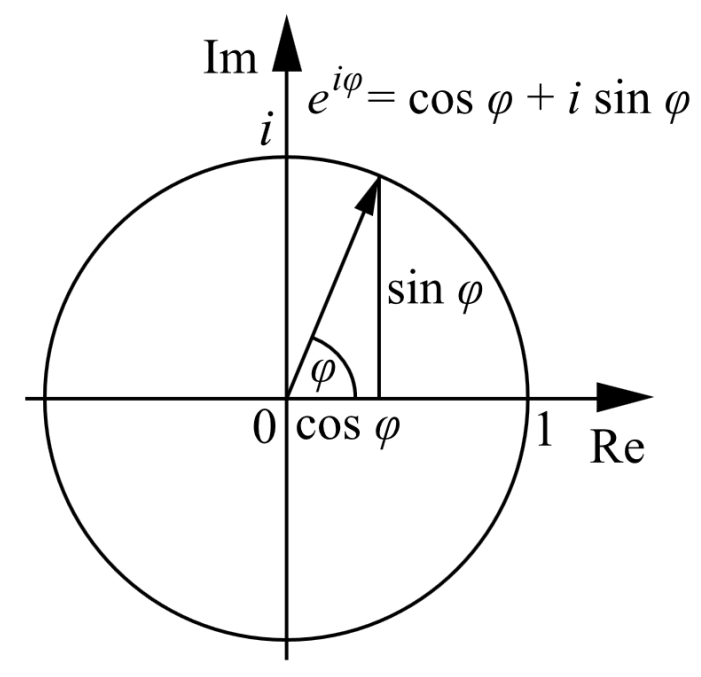
\includegraphics[width=0.5\textwidth]{chap1/img/euler-formula-imaginary-plane.png}
        \caption{$\mathe^{\mathi \varphi}$ 在复平面上的表示}
        \label{fig:euler-formula-imaginary-plane}
    \end{figure}

    如果使 $\varphi$ 随着时间 $t$ 的变化而变化,则画出三维图像(纵轴为时间)
    如图 \ref{fig:euler-formula-imaginary-signals.png} 所示。
    \begin{figure}[H]
        \centering
        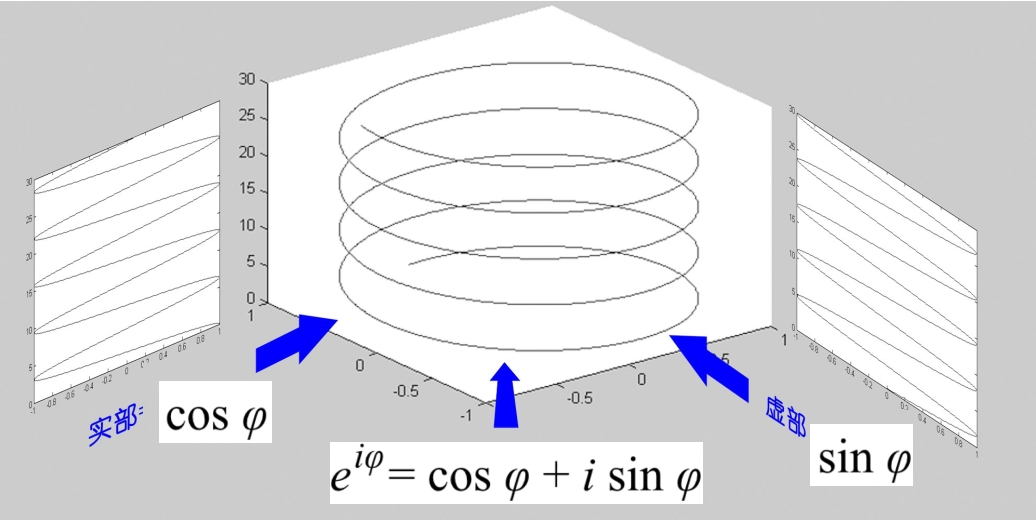
\includegraphics[width=0.5\textwidth]{chap1/img/euler-formula-imaginary-signals.png}
        \caption{$\mathe^{\mathi \varphi}$ 随时间的变化的在三维空间中的轨迹}
        \label{fig:euler-formula-imaginary-signals.png}
    \end{figure}
\end{example}

\begin{example}[复值信号在电磁场中的应用]
    由于电场和磁场互相垂直,所以可以用复值信号的实数部分和虚数部分分别表示电场与磁场信号。
\end{example}

\begin{proof}
    (欧拉公式的微分法证明) 设有函数
    \begin{align*}
        f(x) = \frac{\cos x + \mathi \sin x}{\mathe^{\mathi x}}.
    \end{align*}
    则
    \begin{align*}
        \frac{\D{f}}{\D{x}} & = \frac{(-\sin x + \mathi \cos x)\mathe^{\mathi x}
                    - (\cos x + \mathi \sin x)\mathi \mathe^{\mathi x}}
                    {\mathe^{2\mathi x}} \\
        & = \frac{\mathe^{\mathi x}(-\sin x + \mathi \cos x - \mathi \cos x + \sin x)}{\mathe^{2\mathi x}} \\
        & = 0.
    \end{align*}
    因此 $f(x)$ 为常函数,故 $f(x) = f(0) = 1$。
    此即 $\mathe^{\mathi x} = \cos x + \mathi \sin x$。
\end{proof}

\begin{definition}[复指数信号]
    形如 $f(t) = K\mathe^{st}$,其中 $K \in \set{R}, s \in \set{C}$ 为参数,$t \in \set{R}$ 为自变量,
    这样的信号被称为\bd{复指数信号}。
\end{definition}

\begin{property}[复指数信号与正余弦信号之间的关系]
    不妨设 $s = \sigma + \mathi\omega$,其中 $\sigma, \omega \in \set{R}$。则复指数信号
    \begin{align*}
        f(t) & = K\mathe^{st} \\
        & = K\mathe^{(\sigma + \mathi\omega)t} \\
        & = K\mathe^{\sigma t} \cdot \mathe^{\mathi \omega t} \\
        & = K\mathe^{\sigma t} \cdot (\cos \omega t + \mathi \sin \omega t).
    \end{align*}

    固定 $K, \sigma, \omega$ 中的两个,做出第三个关于 $t$ 的变化图像如下:
    \begin{itemize}
        \item 固定 $\sigma = 0.2, \omega = 1$,$K$ 变化:图 \ref{fig:complex-exponential-signal-k-vary}。
        \item 固定 $K = 1, \omega = 1$,$\sigma$ 变化:图 \ref{fig:complex-exponential-signal-sigma-vary}。
        \item 固定 $K = 1, \sigma = 0.2$,$\omega$ 变化:图 \ref{fig:complex-exponential-signal-omega-vary}。
    \end{itemize}
    \begin{figure}[H]
        \centering
        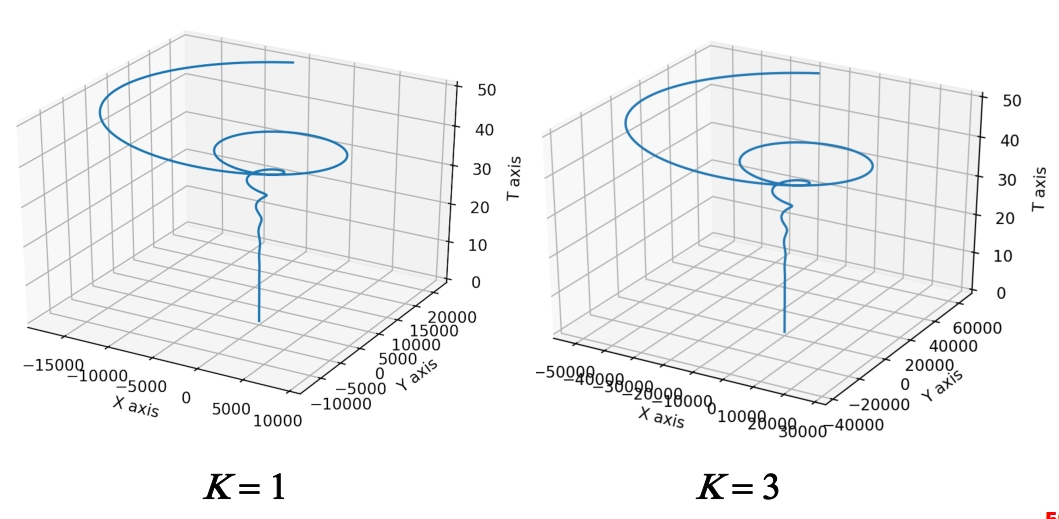
\includegraphics[width=0.5\textwidth]{chap1/img/complex-exponential-signal-k-vary.png}
        \caption{固定 $\sigma = 0.2, \omega = 1$,$K$ 变化}
        \label{fig:complex-exponential-signal-k-vary}
    \end{figure}
    \begin{figure}[H]
        \centering
        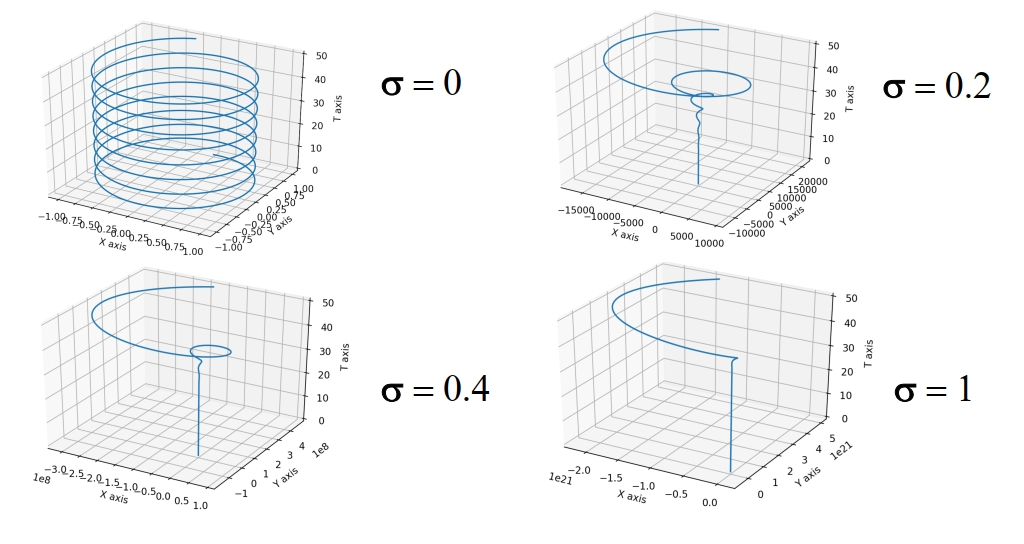
\includegraphics[width=0.5\textwidth]{chap1/img/complex-exponential-signal-sigma-vary.png}
        \caption{固定 $K = 1, \omega = 1$,$\sigma$ 变化}
        \label{fig:complex-exponential-signal-sigma-vary}
    \end{figure}
    \begin{figure}[H]
        \centering
        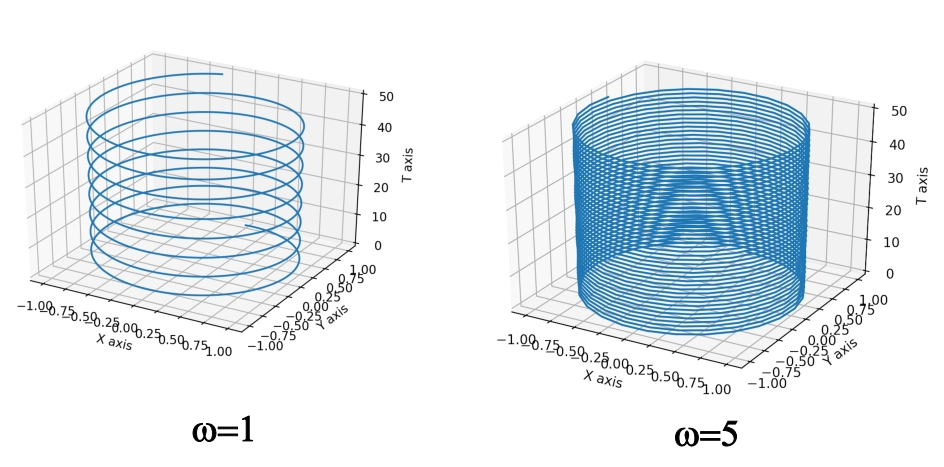
\includegraphics[width=0.5\textwidth]{chap1/img/complex-exponential-signal-omega-vary.png}
        \caption{固定 $K = 1, \sigma = 0.2$,$\omega$ 变化}
        \label{fig:complex-exponential-signal-omega-vary}
    \end{figure}
\end{property}

\subsubsection{函数分解}

\begin{definition}[正交基]
    设 $V$ 为欧式空间,非零向量 $\alpha_1, \alpha_2, \cdots, \alpha_m \in V$。
    \begin{enumerate}
        \item 如果它们两两正交,则称之为\bd{正交向量组}。
            一个较为显然的事实是,$n$ 维欧式空间中正交向量组所含向量个数 $\le n$。
        \item $n$ 维欧式空间中,由 $n$ 个向量构成的正交向量组称为\bd{正交基}。
        \item 由单位向量构成的正交基称为\bd{标准正交基}。
    \end{enumerate}
\end{definition}

\begin{example}
    在标准欧式空间 $\set{R}^3$ 中,向量组
    \begin{align*}
        \beta_1 = (0, 1, 0),
        \quad \beta_2 = (\frac{\sqrt{2}}{2}, 0, \frac{\sqrt{2}}{2}),
        \quad \beta_3 = (\frac{\sqrt{2}}{2}, 0, -\frac{\sqrt{2}}{2})
    \end{align*}
    是一个标准正交基。这是因为
    \begin{align*}
        \beta_1 \cdot \beta_2 = \beta_1 \cdot \beta_3 = \beta_2 \cdot \beta_3 = 0,
    \end{align*}
    且
    \begin{align*}
        \|\beta_1\| = \|\beta_2\| = \|\beta_3\| = 1.
    \end{align*}
\end{example}

\begin{definition}[正交函数与正交函数集]
    在 $[t_1, t_2]$ 区间上定义的非零函数 $\varphi_1(t)$ 与 $\varphi_2(t)$,
    若满足条件
    \begin{align*}
        \int_{t_1}^{t_2}\varphi_1(t)\varphi_2^*(t)\D{t} = 0,
    \end{align*}
    则称函数 $\varphi_1(t)$ 与 $\varphi_2(t)$ 为在 $[t_1, t_2]$ 区间上的\bd{正交函数}。

    在 $[t_1, t_2]$ 区间上定义的非零函数序列 $\varphi_1(t), \varphi_2(t), \cdots, \varphi_n(t)$,
    其中任意两个函数 $\varphi_i(t)$ 与 $\varphi_j(t)$,均满足条件
    \begin{align*}
        \int_{t_1}^{t_2}\varphi_i(t)\varphi_j^*(t)\D{t} = \begin{cases}
            0, & i \ne j, \\
            k_i, & i = j,
        \end{cases}
    \end{align*}
    其中 $k_i$ 为非零常数,则称函数序列 $\varphi_1(t), \varphi_2(t), \cdots, \varphi_n(t)$
    为区间 $[t_1, t_2]$ 上的\bd{正交函数集}。$n$ 可以为有限值,也可以为正无穷。
\end{definition}

\begin{note}
    在证明正交函数、正交函数集时,需要注意以下几点:
    \begin{itemize}
        \item 在说明正交性时,一定要强调是\bd{在某个区间上}的正交性。
        \item 在说明正交函数集时,除了证明不等两个函数的内积为 $0$ 外,
            还要证明相等的函数的内积不为 $0$。
    \end{itemize}
\end{note}

\begin{example}[三角函数集]
    设 $\omega_0 > 0$,则
    \begin{align*}
        \{1, \cos(\omega_0t + \varphi_1), \cos(2\omega_0t + \varphi_2),
            \cdots, \cos(n\omega_0 t + \varphi_n))\}
    \end{align*}
    是在 $[0, \frac{2\pi}{\omega_0}]$ 区间上的正交函数集。
\end{example}

\begin{proof}
    整个证明分为四部分:
    首先,$1$ 与 $\cos(k\omega_0t + \varphi_k), \quad k = 1, 2, \cdots, n$ 正交。
    \begin{align*}
        \int_{0}^{\frac{2\pi}{\omega_0}}1\cos(k\omega_0t + \varphi_k)\D{t}
        = \int_{0}^{\frac{2\pi}{\omega_0}}\cos(k\omega_0t + \varphi_k)\D{t}
        = 0.
    \end{align*}
    其次,$\cos(k_1\omega_0t + \varphi_{k_1})$ 与 $\cos(k_2\omega_0t + \varphi_{k_2})$, 在 $k_1 \ne k_2$ 的条件下正交。
    \begin{align*}
        & \quad \int_{0}^{\frac{2\pi}{\omega_0}}\cos(k_1\omega_0t + \varphi_{k_1})\cos(k_2\omega_0t + \varphi_{k_2})\D{t} \\
        & = \int_{0}^{\frac{2\pi}{\omega_0}}\frac{1}{2}(\cos((k_1\omega_0t + \varphi_{k_1}) + (k_2\omega_0t + \varphi_{k_2})) + \cos((k_1\omega_0t + \varphi_{k_1}) - (k_2\omega_0t + \varphi_{k_2}))) \\
        & = \int_{0}^{\frac{2\pi}{\omega_0}}\frac{1}{2}(\cos((k_1 + k_2)\omega_0t + \varphi_{k_1} + \varphi_{k_2}) + \cos((k_1 - k_2)\omega_0t + \varphi_{k_1} - \varphi_{k_2}))\D{t} \\
        & = \left(\frac{1}{2(k_1 + k_2)\omega_0}\sin((k_1 + k_2)\omega_0t + \varphi_{k_1} + \varphi_{k_2})
            + \frac{1}{2(k_1 - k_2)}\sin((k_1 - k_2)\omega_0t + \varphi_{k_1} - \varphi_{k_2})\right)\Big|_{0}^{\frac{2\pi}{\omega_0}} \\
        & = 0.
    \end{align*}
    再次,$1$ 与自身不正交。
    \begin{align*}
        \int_{0}^{\frac{2\pi}{\omega_0}}1\cdot 1\D{t}
        = \frac{2\pi}{\omega_0} \ne 0.
    \end{align*}
    最后,$\cos(k\omega_0t + \varphi_k)$ 与自身不正交。
    \begin{align*}
        & \quad \int_{0}^{\frac{2\pi}{\omega_0}}\cos^2(k\omega_0t + \varphi_k)\D{t} \\
        & = \int_{0}^{\frac{2\pi}{\omega_0}}\frac{1 + \cos(2k\omega_0t + 2\varphi_k)}{2}\D{t} \\
        & = \frac{\pi}{\omega_0} + \frac{1}{2}\cdot\frac{1}{2k\omega_0}\sin(2k\omega_0t + 2\varphi_k)\Big|_{0}^{\frac{2\pi}{\omega_0}} \\
        & = \frac{\pi}{\omega_0} \ne 0.
    \end{align*}
    因此,$\{1, \cos(\omega_0t + \varphi_1), \cos(2\omega_0t + \varphi_2), \cdots, \cos(n\omega_0 t + \varphi_n))\}$
    是在 $[0, \frac{2\pi}{\omega_0}]$ 区间上的正交函数集。
\end{proof}

\begin{example}[指数函数集]
    设 $\omega_0 > 0$,则
    \begin{align*}
        \{\mathe^{\mathi n\omega_0t} \mid n \in \set{Z}\}
    \end{align*}
    是在区间 $[-\frac{\pi}{\omega_0}, \frac{\pi}{\omega_0}]$ 上的正交函数集。
\end{example}

\begin{proof}
    任取 $m, n \in \set{Z}$。若 $m \neq n$,则 $\mathe^{\mathi m\omega_0t}$ 和 $\mathe^{\mathi n\omega_0t}$
    在区间 $[-\frac{\pi}{\omega_0}, \frac{\pi}{\omega_0}]$ 上正交,这是因为
    \begin{align*}
        \int_{-\frac{\pi}{\omega_0}}^{\frac{\pi}{\omega_0}}\mathe^{\mathi m\omega_0t}\mathe^{-\mathi n\omega_0t}\D{t}
        = \int_{-\frac{\pi}{\omega_0}}^{\frac{\pi}{\omega_0}}\mathe^{\mathi (m - n)\omega_0t}\D{t}
        = \frac{\mathe^{\mathi (m - n)\omega_0t}}{\mathi (m - n)\omega_0}\Big|_{-\frac{\pi}{\omega_0}}^{\frac{\pi}{\omega_0}}
        = 0.
    \end{align*}
    若 $m = n$,则 $\mathe^{\mathi m\omega_0t}$ 和 $\mathe^{\mathi n\omega_0t}$
    在区间 $[-\frac{\pi}{\omega_0}, \frac{\pi}{\omega_0}]$ 上不正交,这是因为
    \begin{align*}
        \int_{-\frac{\pi}{\omega_0}}^{\frac{\pi}{\omega_0}}\mathe^{\mathi m\omega_0t}\mathe^{-\mathi m\omega_0t}\D{t}
        = \int_{-\frac{\pi}{\omega_0}}^{\frac{\pi}{\omega_0}}1\D{t}
        = \frac{2\pi}{\omega_0} \neq 0.
    \end{align*}
    因此 $\{\mathe^{\mathi n\omega_0t} \mid n \in \set{Z}\}$ 是
    在区间 $[-\frac{\pi}{\omega_0}, \frac{\pi}{\omega_0}]$ 上的正交函数集。
\end{proof}

\begin{definition}[完备的正交函数集]
    如果在区间 $[t_1, t_2]$ 上,除了正交函数集 $\{\varphi_i(t)\}$ 之外,不存在函数 $x(t)$,
    满足 $0 < \int_{t_1}^{t_2}x(t)x^*(t)\D{t} < +\infty$,使得
    \begin{align*}
        \int_{t_1}^{t_2}x(t)\varphi_i^*(t)\D{t} = 0, \quad \forall i,
    \end{align*}
    则称此正交函数集 $\{\varphi_i(t)\}$ 为区间 $[t_1, t_2]$ 上的\bd{完备的正交函数集}。
\end{definition}

\begin{remark}
    事实上,指数函数集 $\{\mathe^{\mathi n\omega_0t} \mid n \in \set{Z}\}$ 在
    区间 $[-\frac{\pi}{\omega_0}, \frac{\pi}{\omega_0}]$ 上是完备的正交函数集。
\end{remark}

% \begin{proof}
%     设 $x(t)$ 是在区间 $[-\frac{\pi}{\omega_0}, \frac{\pi}{\omega_0}]$ 上的任意函数。
%     由于 $\{\mathe^{\mathi n\omega_0t} \mid n \in \set{Z}\}$ 是正交函数集,因此
%     \begin{align*}
%         \int_{-\frac{\pi}{\omega_0}}^{\frac{\pi}{\omega_0}}x(t)\mathe^{\mathi n\omega_0t}\D{t} = 0, \quad \forall n \in \set{Z}.
%     \end{align*}
%     由此可得
%     \begin{align*}
%         x(t) = \sum_{n = -\infty}^{+\infty}c_n\mathe^{\mathi n\omega_0t},
%     \end{align*}
%     其中 $c_n = \frac{1}{2\pi}\int_{-\frac{\pi}{\omega_0}}^{\frac{\pi}{\omega_0}}x(t)\mathe^{-\mathi n\omega_0t}\D{t}$。
%     因此 $\{\mathe^{\mathi n\omega_0t} \mid n \in \set{Z}\}$ 是在区间 $[-\frac{\pi}{\omega_0}, \frac{\pi}{\omega_0}]$ 上的完备的正交函数集。
% \end{proof}
